% imports 
\section{Overview}
Previous solutions to the bus charge problem have all struggled with scalability. In this work, we provide a solution which not only manages the monthly cost of power and adheres to the operational constraints of a bus fleet, but also scales to a large number of buses by segmenting the problem into a series of subproblems. Each subploblem is solved using a linear, quadratic, or integer program, and when used together the series of programs provides a cost-oriented charge plan. 
\par The charge problem is solved in eight steps as shown in Figures \ref{fig:processChain} and \ref{fig:groupProcessing}.  The first step solves an unconstrained problem where each bus is assumed to have a dedicated charger, eliminating the need for contention. Because optimizers tend to work along the edges of a feasible set, this first solution tends to yield charge schedules that command on-off solutions, which require that a charger either charge at zero, or its maximum rate which can be difficult to implement in reality. 
\par We desire to achieve a smooth solution without sacrificing cost. The second problem resolves the original problem with two differences. The first is that the solution {\it must} match the optimal cost given in the first solution. The second is to replace the original objective with an objective that incentivises a smooth solution.
\par So far the smooth solution does not account for limited numbers of chargers, however assigning buses to chargers is a non-convex and significantly increases computations. Before we address the assignment problem, we separate buses into groups so that the group-wise computations are manageable. The next several steps are computed separately for each group as shown in Fig. \ref{fig:groupProcessing}.  
\par Up to this point, we have computed an ``ideal'', ``smooth'' solution and separated buses into groups of manageable size. Before we can assign buses to chargers we require that charge sessions deliver a minimum energy so that the burden of connecting is worth while. The process of reallicating energy is referred to as ``de-fragmentation'' and yields another charge schedule that still assumes one charger per bus.
\par Now we know at which rest periods a bus must charge and how much energy must be delivered.  The next problem is to assign buses to chargers and manage contention so that multiple buses are not simultaneously assigned to the same charger. However, the bus assignment problem can require significant computations and may require a large gap to manage computation times. Because the gap may be large, the route schedules may require addional changes to maximize a bus's time on a charger which is addressed be the session refinement problem. 
\par Once sessions have been refined, we know at which rest periods a bus must charge, how much energy must be delivered, at which charger a bus will charge, and when that bus is scheduled to charge. The next step is to compute a minute-by-minute charge schedule for each bus which plans how energy will be delivered as a function of time which is referred to as the ``Constrained Optimzation'' problem. 
\par Solutions from the Constrained Optimization problem tend to favor non-smooth solutions for the same reasons as the Unconstrained Optimal solution. Therefore, the final step is to compute a smoothed version of the optimal solution which maintians the optimal cost while minimising large jumps in power between time steps as was done in the ``Unconstrained Smoothing'' problem.
\begin{figure*}\centering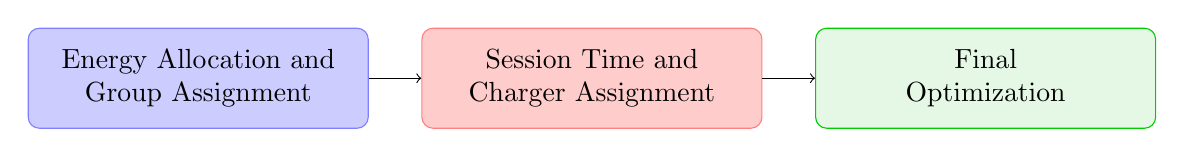
\begin{tikzpicture}
	\node[rectangle, draw=blue!50, fill=blue!20, minimum width=1.7in, minimum height=0.5in, rounded corners](set1) at (0,0) {\begin{tabular}{c} Energy Allocation and\\ Group Assignment\end{tabular}}; 
	\node[rectangle, draw=red!50, fill=red!20, minimum width=1.7in, minimum height=0.5in, rounded corners](set2) at (5,0) {\begin{tabular}{c} Session Time and \\Charger Assignment \end{tabular}}; 
	\node[rectangle, draw=green!80!black, fill=green!70!black!10, minimum width=1.7in, minimum height=0.5in, rounded corners](set3) at (10,0) {\begin{tabular}{c} Final \\ Optimization\end{tabular}}; 
	\draw[->] (set1.east) -- (set2.west);
	\draw[->] (set2.east) -- (set3.west);
\end{tikzpicture}\caption{Overall Processing Chain}\label{fig:processChain}\end{figure*}


\begin{figure*}\centering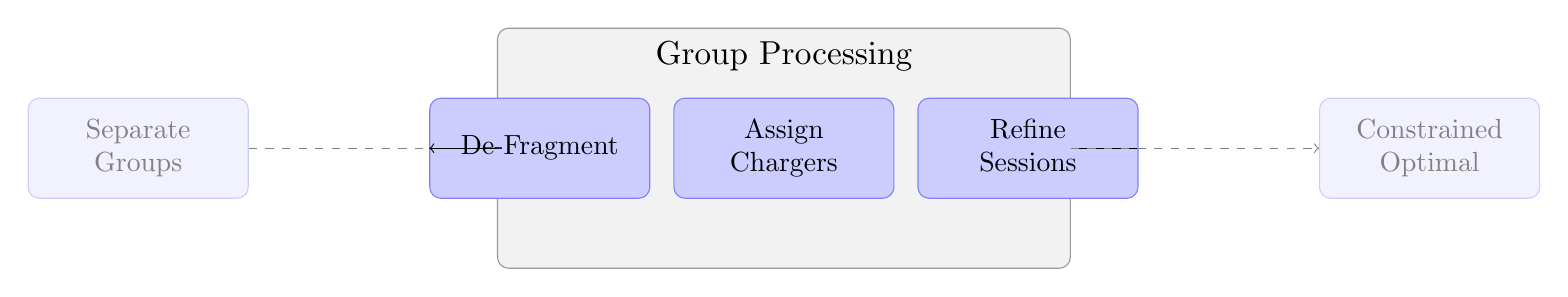
\begin{tikzpicture}
\node[rectangle, draw=gray!80, fill=gray!10, minimum width=\textwidth*0.6, minimum height=1.2in, rounded corners, label={[label distance=-0.67cm]above:\scalebox{1.2}{Group Processing}}](outline) at (0,0){};
	\node[rectangle, draw=blue!50, fill=blue!20, minimum width=1.1in, minimum height=0.5in, rounded corners](problem1) at (-3.1,0) {De-Fragment}; 
	\node[rectangle, draw=blue!50, fill=blue!20, minimum width=1.1in, minimum height=0.5in, rounded corners](problem2) at (0,0) {\begin{tabular}{c}Assign\\ Chargers\end{tabular}}; 
	\node[rectangle, draw=blue!50, fill=blue!20, minimum width=1.1in, minimum height=0.5in, rounded corners](problem3) at (3.1,0) {\begin{tabular}{c}Refine\\ Sessions\end{tabular}}; 
	\node[rectangle, draw=blue!20, fill=blue!5, text=black!50, minimum width=1.1in, minimum height=0.5in, rounded corners](problem0) at (-8.2,0){\begin{tabular}{c}Separate \\ Groups \end{tabular}};
	\node[rectangle, draw=blue!20, fill=blue!5, text=black!50, minimum width=1.1in, minimum height=0.5in, rounded corners](problem4) at (8.2,0){\begin{tabular}{c}Constrained\\ Optimal\end{tabular}};
	\draw[draw=black!50, dashed] (problem0.east) -- (outline.west);
	\draw[->] (outline.west) -- (problem1.west);
	\draw (problem3.east) -- (outline.east);
	\draw[->, draw=black!50, dashed] (outline.east) -- (problem4.west);
\end{tikzpicture}\caption{Processing chain for each group} \label{fig:groupProcessing}\end{figure*}


\section{Scheduling an Optimal Solution\label{sec:optimalSolution}}
This section describes a program that finds an optimal charge schedule where buses are allowed to charge without regard to the number of available chargers. This solution is considered ``optimal'' and will be used in later sections to formulate a feasible solution that accounts for the number of chargers.
\begin{table*}
\centering
\caption{Description of the billing structure}
\begin{tabular}{c | c c c}
		                   & On-Peak                & Off-Peak               & Facilities (Both)\\ \hline
		Energy Rate        & \$ 0.058282  /kWh & \$ 0.029624 /kWh  & None \\
		Energy Rate Symbol & $\mu_{\text{e-on}}$    & $\mu_{\text{e-off}}$   & None \\ \hline
		Power Rate  & \$ 15.73 /kW           & None                   & \$ 4.81 /kW \\
		Power Rate Symbol  & $\mu_{\text{p-on}}$    & None            & $\mu_{\text{p-all}}$
	\end{tabular}
	\label{tab:charges} 
\end{table*}

 
\begin{figure*}
\centering
\scalebox{0.8}{
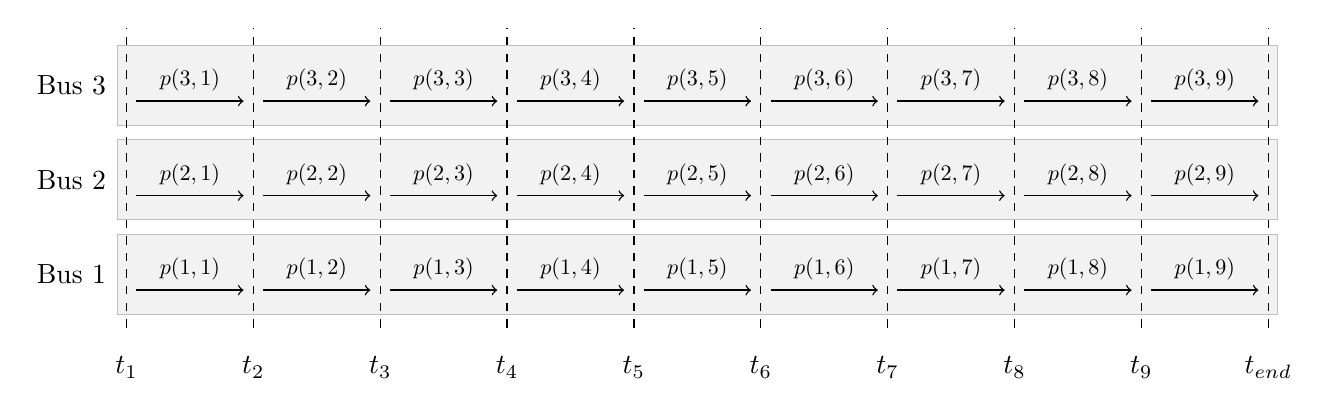
\begin{tikzpicture}
	\node[rectangle, draw=gray!50, fill=gray!10, minimum width=5.8in, minimum height=0.4in](bus1Box) at (7.75,0.8){};
	\node(bus1BoxLabel) at (-0.2, 0.8){Bus 1}; 
	
	\node[rectangle, draw=gray!50, fill=gray!10, minimum width=5.8in, minimum height=0.4in](bus2Box) at (7.75,2){};
	\node(bus1BoxLabel) at (-0.2, 2.0){Bus 2};
	
	\node[rectangle, draw=gray!50, fill=gray!10, minimum width=5.8in, minimum height=0.4in](bus3Box) at (7.75,3.2){};
	\node(bus1BoxLabel) at (-0.2, 3.2){Bus 3};
	
	\foreach \curLab/\preLab[count=\c, evaluate=\c as \pos using {0.5 + (\c - 1)*14.5/9}] in {t_1/t_1, t_2/t_1, t_3/t_2, t_4/t_3, t_5/t_4, t_6/t_7, t_7/t_6, t_8/t_7, t_9/t_8, t_{end}/t_9}
	{
		\node[label=below:$\curLab$](b\c) at (\pos, 0){};
		\node(t) at (\pos, 3.8){};
		\draw[dashed, line width=0.5pt] (b\c.north) -- (t.north); 
		\ifnum\c>1 
			\node(b1Curr) at (\pos, 0.8 - 0.2){};
			\node(b2Curr) at (\pos, 2.0 - 0.2){};
			\node(b3Curr) at (\pos, 3.2 - 0.2){};
			\def\temp{\number\numexpr\c - 1}
			\draw[->, line width=0.5pt] (b1Prev.east) -- node[midway, above]{\scalebox{0.8}{$p(1,\temp)$}}(b1Curr.west);
			\draw[->, line width=0.5pt] (b2Prev.east) -- node[midway, above]{\scalebox{0.8}{$p(2,\temp)$}}(b2Curr.west);
			\draw[->, line width=0.5pt] (b3Prev.east) -- node[midway, above]{\scalebox{0.8}{$p(3,\temp)$}}(b3Curr.west);	
		\fi
			\node(b1Prev) at (\pos, 0.8 - 0.2){};
			\node(b2Prev) at (\pos, 2.0 - 0.2){};
			\node(b3Prev) at (\pos, 3.2 - 0.2){};	
	}
	\path (b9.south) -- node[midway, below=0.1in]{$\hdots$}(b10.south);

\end{tikzpicture}}
\caption{Demonstrates how bus power use is conceptualized}
\label{fig:busPower}
\end{figure*}


\begin{figure*}
\centering
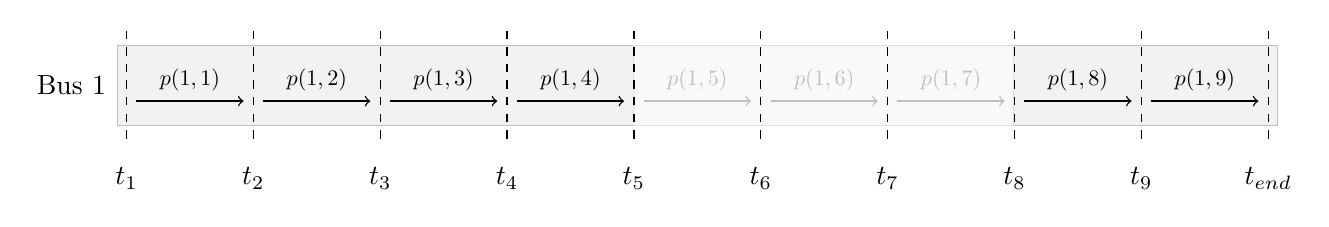
\begin{tikzpicture}
	\node[rectangle, draw=gray!50, fill=gray!10, minimum width=5.8in, minimum height=0.4in](bus1Box) at (7.75,0.8){};
	\node(bus1BoxLabel) at (-0.2, 0.8){Bus 1}; 
	\node[rectangle, draw=gray!25, fill=gray!5, minimum width=1.9in, minimum height=0.4in](bus1Box) at (7.75 + 1.6,0.8){};
	
	\foreach \curLab/\preLab[count=\c, evaluate=\c as \pos using {0.5 + (\c - 1)*14.5/9}] in {t_1/t_1, t_2/t_1, t_3/t_2, t_4/t_3, t_5/t_4, t_6/t_5, t_7/t_6, t_8/t_7, t_9/t_8, t_{end}/t_9}
	{
		\node[label=below:$\curLab$](b\c) at (\pos, 0){};
		\node(t) at (\pos, 1.4){};
		\ifnum\c>1 
			\node(b1Curr) at (\pos, 0.8 - 0.2){};
				\ifnum\c > 5
					\ifnum\c < 9 
						\def\clr{black!25}
					\else
						\def\clr{black}
					\fi
				\else
					\def\clr{black}
				\fi
				\draw[->, line width=0.5pt, \clr] (b1Prev.east) -- node[midway, above]{\scalebox{0.8}{$p(1,\number\numexpr\c-1)$}}(b1Curr.west); 
		\fi
		\node(b1Prev) at (\pos, 0.8 - 0.2){};
		\draw[dashed, line width=0.5pt] (b\c.north) -- (t.north); 
	}
	\path (b9.south) -- node[midway, below=0.1in]{$\hdots$}(b10.south);

\end{tikzpicture}
\caption{Bus schedule with availability}
\label{fig:busAvail}
\end{figure*}

 
\subsection{Formulation\label{sec:formulation}} 
The cost objective that we desire to minimize is modeled after \cite{rocky_mountain_power_rocky_2021}, which contains two primary elements: the cost of energy, and power demand. Energy is billed per kWh for on-peak and off-peak hours. The on-peak rate is more expensive because there is generally more demand for power during this time, whereas off-peak hours tend to be less expensive. The demand is covered in two separate chargers.  The first is a facilities charge which is billed per kW for the highest 15-minute average power use over the course of the month. The second is a demand charge, which is also billed per kW, but is only billed for the highest 15-minute average power usesd during on-peak hours. The rates for each component are given in Table \ref{tab:charges}.  

Before we may compute the total monthly cost of electricity, we must define expressions for the average power and energy over time.  Let each day be divided into 15-minute intervals for each bus where the average power expended for bus $i$ during time $j$ is denoted $p(i,j)$ as shown in Fig. \ref{fig:busPower}. The resulting solution of the program we will develop will yield the average power expended by each bus during each period of time.
\par One constraint for which the solution must account is bus availability.  When a bus is out of the station, the maximum average power for that time must be zero. For example, if bus 1 were out on route for $t_5, t_6,$ and $t_7$, then the average power for those periods would be equal to zero as shown in Fig. \ref{fig:busAvail}. Let $\bm{b}_{p(i,j)}$ be the average power used by bus $i$ at time index $j$, and $\bm{b}$ be a vector which contains $b_{p(i,j)}$ for each bus and time index. Also let $\mathcal{A} \subset {i\times j}$  be the set of all indices where bus $i$ is in the station during time $t_j$ and $\tilde{\mathcal{A}}$ be its complement. Furthermore, let $p_{\text{max}}$ be the maximum power that a charger can deliver. 
\par We define a set of constraints so that buses do not use power when not in the station by letting
\begin{equation}\label{eqn:obj:power1}\begin{aligned}
	b_{p(i,j)} &= 0 \ \forall i,j \in \tilde{\mathcal{A}}  \\
	b_{p(i,j)} &\le p_{\text{max}} \ \forall i,j \in \mathcal{A} \\
	-b_{p(i,j)} &\le 0              \ \forall i,j \in \mathcal{A} 
\end{aligned}\end{equation}
\par The constraints in Eq. \ref{eqn:obj:power1} however to not account for buses that must charge for partial periods.  For example, if the day were divided into 15-minute time blocks, but a bus began charging at 10:07, then an average power of $p_{\text{max}}$ for that time slot would be inaccurate. Therefore, Eq. \ref{eqn:obj:power1} must be modified so that the average power for each block correctly reflects partial availability.  Let $\alpha(i,j)$ give the percentage of time that bus $i$ is available during time $j$. Eq. \ref{eqn:obj:power1} can be rewritten as
\begin{equation}\label{eqn:obj:power2}\begin{aligned}
	-b_{p(i,j)} &\le 0 \ \forall i,j \\
	b_{p(i,j)}  &\le p_{\text{max}}\cdot \alpha(i,j) \ \forall  i,j\\
\end{aligned}\end{equation}



